\documentclass[10pt]{examdesign}
\usepackage{amsmath}
\usepackage{enumitem}
\usepackage{amsfonts}
\usepackage{pgfplots}
\usepackage{pifont}
\usepackage{graphicx}
\usepackage{fancyhdr}
\usepackage{cancel}


\SectionFont{\large\sffamily}
\Fullpages
\ContinuousNumbering
\usepackage{ulem}
\ProportionalBlanks{2}


\DefineAnswerWrapper{}{}
\NumberOfVersions{1}
%\IncludeFromFile{foobar.tex}
\examname{\Large{Waves Quiz}}
\class {\Large Physics}

\def \namedata {Name: \hrulefill\\ 
	Date: \hrulefill \\
	Period: \hrulefill \\
	Peer Reviewer: \hrulefill \\
	Authentication Code: \hrulefill
	\\
		
	\begin{tabular}{| p{1cm} | p{1cm} | p{1 cm} | p{1cm} |}
	\hline
		+1 & 0 & -1 & $\Sigma$ 
		\\
		\hline
		& & & \vspace{.5cm}
		\\ \hline
	
	\end{tabular}
	\\
 \vspace{-.6in}
	
}




\begin{document}




\begin{multiplechoice} [title={Multiple Choice},
	rearrange=no]
	\textit{Choose the best answer to each question.} 


\begin{block}
	
Questions 1-4 Refer to the following information:

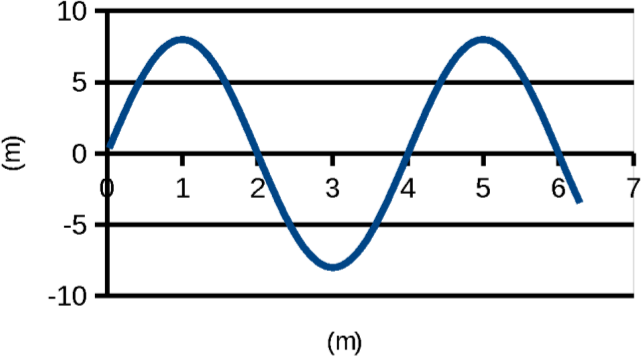
\includegraphics[width=3in]{wave.png}
 
	\begin{question}
	What is the wavelength of the wave shown above?
	\choice {2 m}
	\choice [!]{4 m}
	\choice{6 m}
	\choice {7.5 m}
	\choice {15 m}
\end{question}

	\begin{question}
What is the amplitude of the wave shown above?
	\choice {2 m}
	\choice {4 m}
	\choice{6 m}
	\choice [!]{7.5 m}
	\choice {15 m}
\end{question}

	
\begin{question}
	The wave pictured above is best described as a(n) - 
	\choice [!]{transverse wave}
	\choice {longitudinal wave}
	\choice {electromagnetic wave}
	\choice {A sound wave}
\end{question}


\end{block} 

\begin{question}
	The wave has a period of 0.5 s.  What is its frequency?
	\choice{5 Hz}
	\choice[!]{2 Hz}
	\choice{1 Hz}
	\choice{0.5 Hz}
\end{question}

\begin{block}

	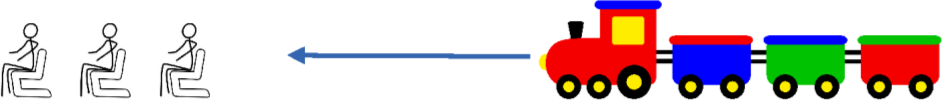
\includegraphics[width=5in]{train.png} 


\begin{question}
	A train is approaching a train station where several students are sitting in chairs, as shown above.  If the train's whistle has a frequency of 700 Hz, the frequency the people hear is - 
		\choice[!]{Greater than 700 Hz} 
		\choice{Exactly 700 Hz}
		\choice{Less than 700 Hz}
		\choice{Each person hears a different frequency.}
\end{question}
\end{block}

\begin{question}
	Many freeways are designed with “rumble strips” - a series of grooves on the shoulder of the road that are designed to make noise when a vehicle drifts off the road.  If a vehicle is traveling 30 m/s when it drifts onto one of these rumble strips and hears a frequency of 300 Hz, what is the distance between the center of each groove?
	\choice{9000 m}
	\choice{270 m}
	\choice{10 m}
	\choice[!]{0.1 m}
%	\vspace{1in}
\end{question}

\begin{question}
		Four tuning forks are labeled 128 Hz, 256 Hz, 440 Hz, and 512 Hz.  If all of the tuning forks are made out of the same material, which tuning fork would you expect to be the biggest size?
	\choice{512 Hz}
	\choice{440 Hz}
	\choice{256 Hz}
	\choice[!]{128 Hz}
\end{question}

\begin{question}
A wave on a slinky has a frequency of 4 Hz and travels at a speed of 2 m/s.  What is the wavelength of this wave?
\choice{0.5 m}
\choice[!]{2 m}
\choice{8 m}
\choice{16 m}
\end{question}

\begin{question}
What does the speed of a wave depend on?
	\choice{The frequency and wavelength of the wave.}
	\choice{The period of the wave.}
	\choice{The material it travels in.}
	\choice{The energy that the wave carries.}
\end{question}


\begin{question}
Light is best described as a - 
	\choice{Transverse Wave}
	\choice{Longitudinal Wave}
	\choice{Electromagnetic Wave}
	\choice{Tidal Wave}
	\end{question}



\end{multiplechoice}





\end{document}


